% A simple graph with straight and bend arrows and loops
% Stefan Kottwitz
\documentclass{article}
\usepackage{tikz}
\usetikzlibrary{arrows}
\begin{document}
\section*{Exercise 1}

We have the following markov model:

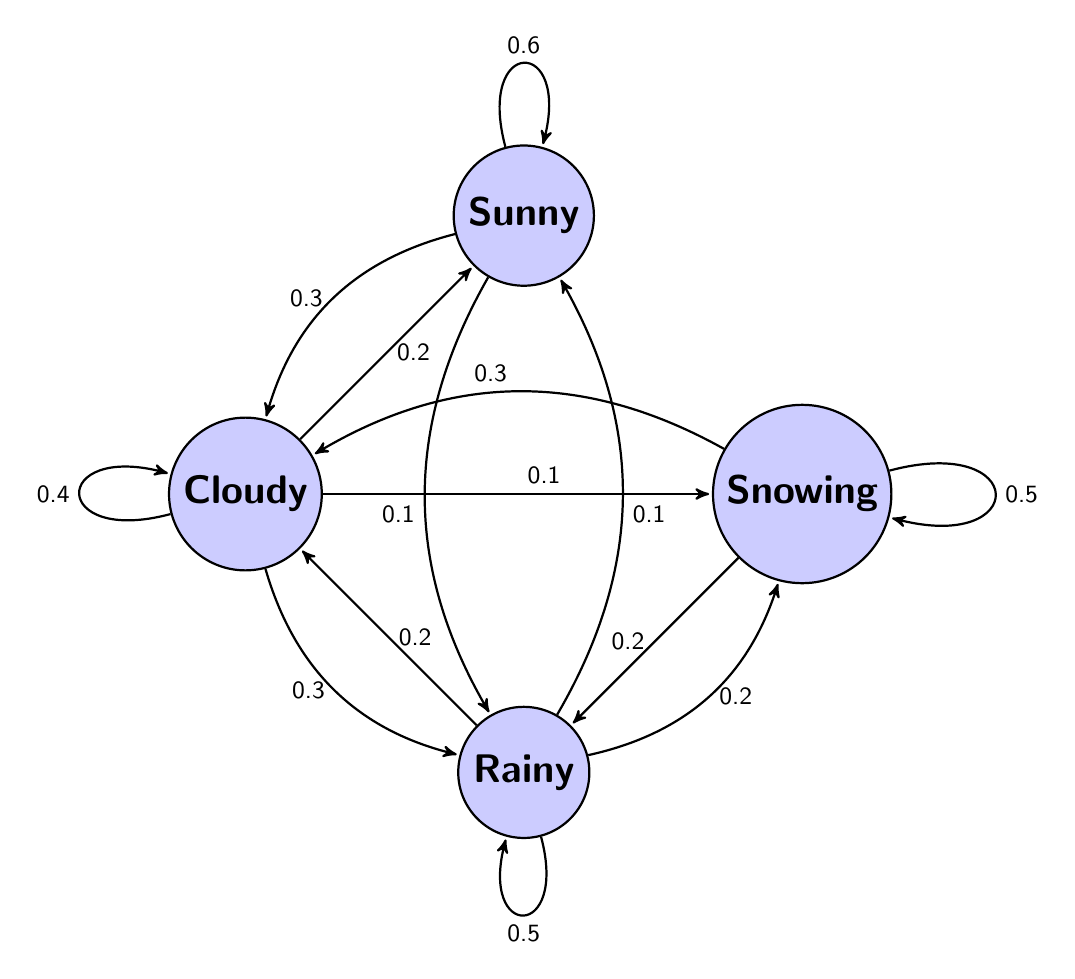
\begin{tikzpicture}[->,>=stealth',shorten >=1pt,auto,node distance=5cm,
  thick,main node/.style={circle,fill=blue!20,draw,font=\sffamily\Large\bfseries}]

  \tikzstyle{pathtaken} = [draw,line width=5pt,-,red!50]

  \node[main node] (1) {Sunny};
  \node[main node] (2) [below left of=1] {Cloudy};
  \node[main node] (3) [below right of=2] {Rainy};
  \node[main node] (4) [below right of=1] {Snowing};

  \path[every node/.style={font=\sffamily\small}]
    (1) % edge node [left] {0.0} (4) %snowing
    	edge [bend right] node [below left] {0.1} (3) %rainy
        edge [bend right] node[left] {0.3} (2) % cloudy
        edge [loop above] node {0.6} (1) % stay sunny
    (2) edge node [right] {0.2} (1)
        edge [loop left] node {0.4} (2)
        edge [bend right] node [left] {0.3} (3)
        edge node [above right] {0.1} (4)
    (3) edge [bend right] node [below right] {0.1} (1)
    	edge node [right] {0.2} (2)
    	edge [loop below] node {0.5} (3)
        edge [bend right] node[right] {0.2} (4)
    (4) edge [bend right] node [above left] {0.3} (2)
    	edge node [left] {0.2} (3)
        edge [loop right] node {0.5} (4);
\end{tikzpicture}
By simply tracing the path and multiplying up the probabilities, we can compute the
probability of a whole sequence $s_1 = $ \{cloudy, rainy, sunny, sunny\}
\begin{equation}
	p(s_1) = 1 \cdot 0.3 \cdot 0.1 \cdot 0.6 = 0.018
\end{equation}
and for the second sequence $s_2 = $ \{sunny, snowy, sunny, rainy\}
\begin{equation}
	p(s_2) = 1 \cdot 0 \cdot 0 \cdot 0.1 = 0
\end{equation}

\section*{Exercise 2}
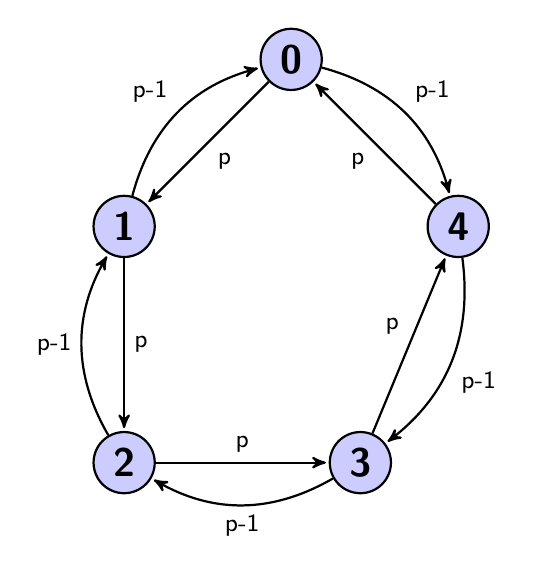
\begin{tikzpicture}[->,>=stealth',shorten >=1pt,auto,node distance=3cm,
  thick,main node/.style={circle,fill=blue!20,draw,font=\sffamily\Large\bfseries}]

  \tikzstyle{pathtaken} = [draw,line width=5pt,-,red!50]

  \node[main node] (0) {0};
  \node[main node] (1) [below left of=0] {1};
  \node[main node] (2) [below of=1] {2};
  \node[main node] (3) [right of=2] {3};
  \node[main node] (4) [below right of=0] {4};
  \path[every node/.style={font=\sffamily\small}]
    (0) edge node {p} (1) 
    	edge [bend left] node {p-1} (4)
    (1) edge node {p} (2) 
    	edge [bend left] node {p-1} (0)    
    (2) edge node {p} (3) 
    	edge [bend left] node {p-1} (1)
    (3) edge node {p} (4) 
    	edge [bend left] node {p-1} (2)
    (4) edge node {p} (0) 
    	edge [bend left] node {p-1} (3);
\end{tikzpicture}

\end{document}